
\subsubsection*{Time-series Embedding}

The \texttt{DataEmbedding}, denoted as $\mathbf{E}$, combines three embeddings to form a robust representation of time-series input sequence. The \texttt{Value Embedding} maps raw input values to a higher-dimensional space via a convolutional layer, capturing intricate data patterns of the input sequence. The \texttt{Positional Embedding} encodes the sequence order using sinusoidal functions, preserving structural information crucial for time-series analysis. The \texttt{Temporal Embedding} incorporates time-related features (e.g., hour, day) to provide context on temporal dependencies and seasonal trends. These components are summed to produce the final embedding matrix $\mathbf{E}$, as described in the equation:

\begin{equation}
\mathbf{E} = \mathbf{E}_{\text{value}} + \mathbf{E}_{\text{position}} + \mathbf{E}_{\text{temporal}} \in \mathbb{R}^{d_x \times d_{\text{embed}}}.
\end{equation}

This matrix serves as the input to the subsequent layers of the model, encapsulating both the intrinsic data patterns and the temporal structure of the time-series.

\subsubsection*{Introduction to Attention Mechanism}

\begin{figure}
\centering
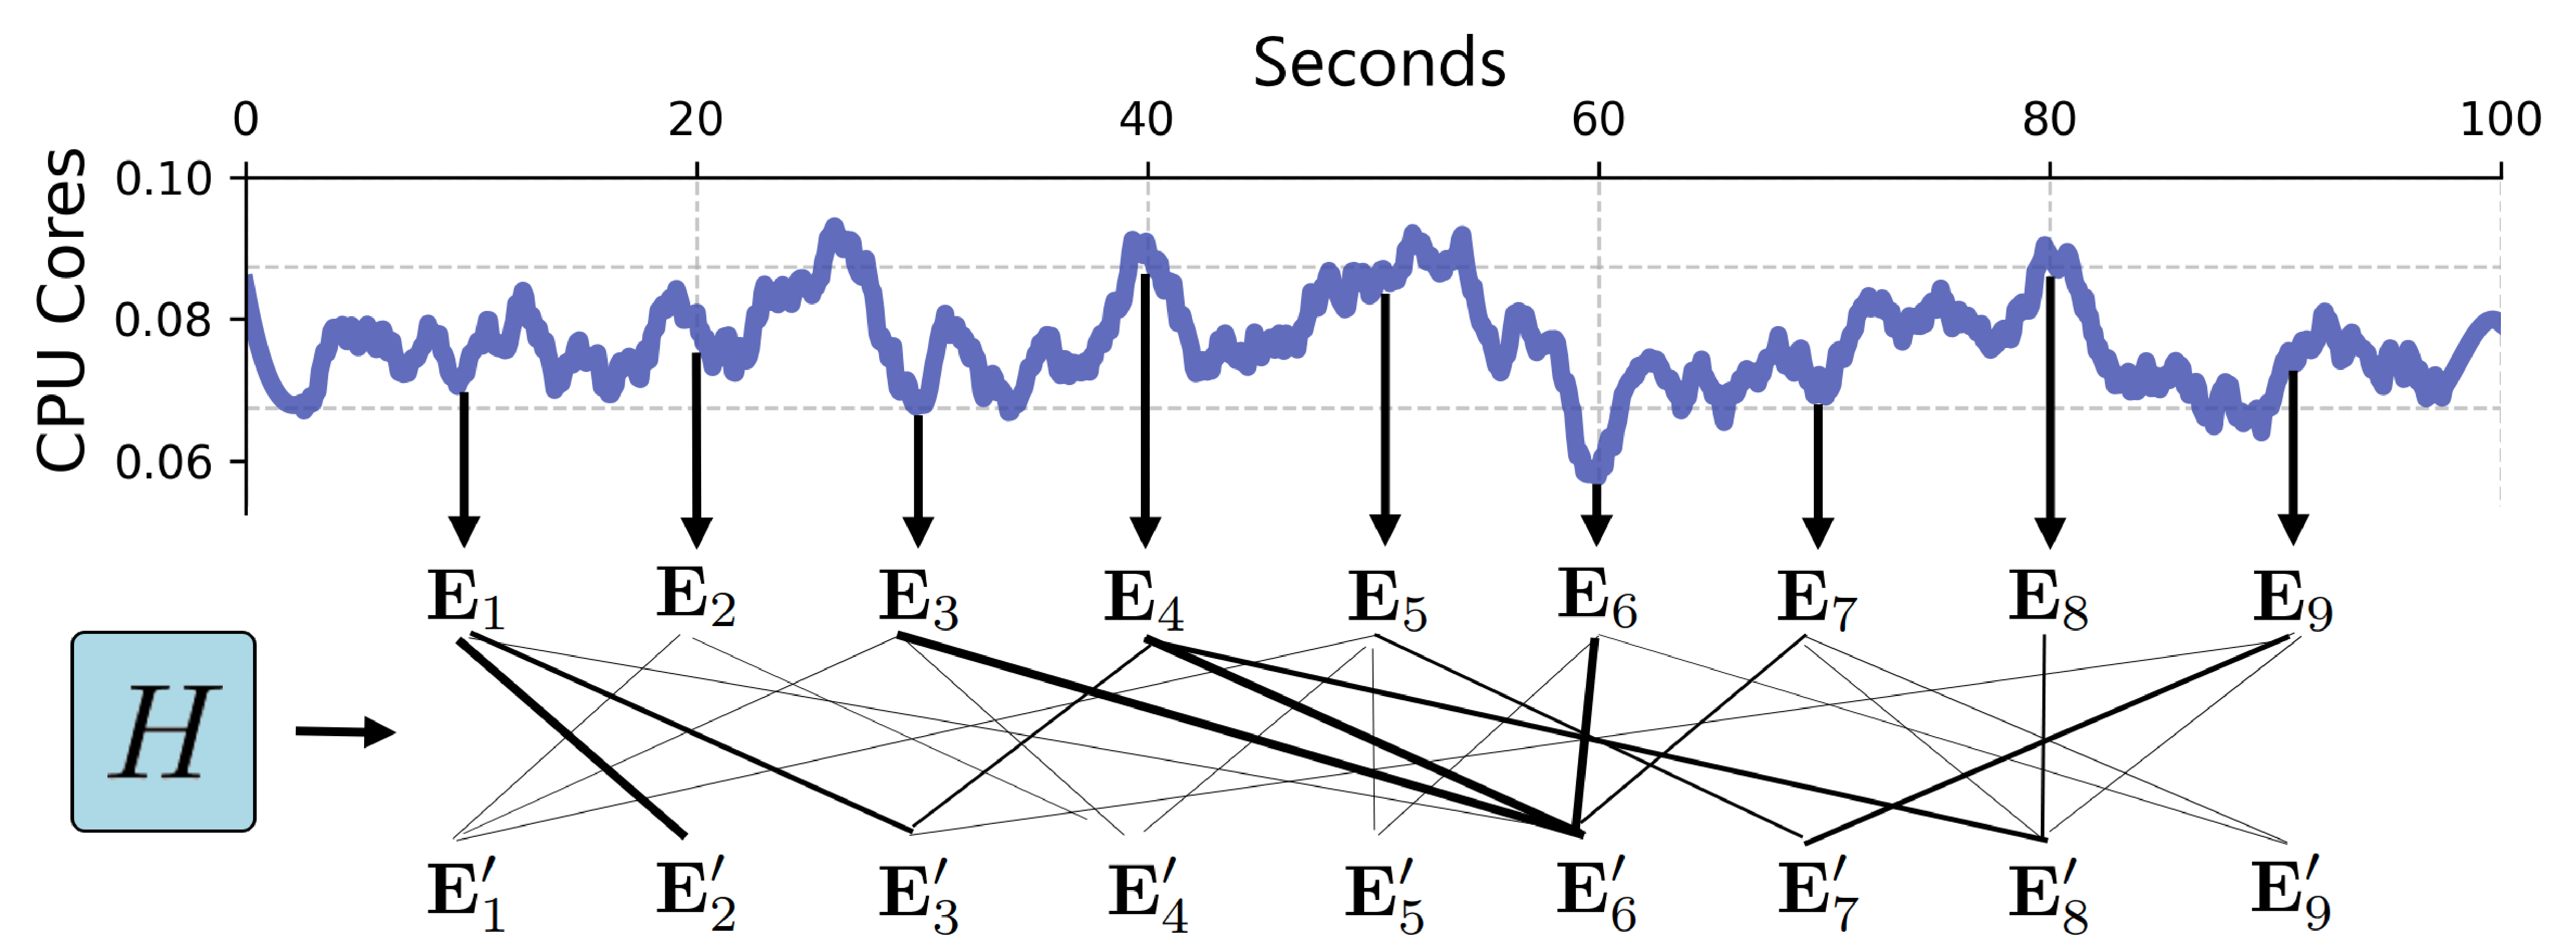
\includegraphics[width=0.49\textwidth]{img/attention_goal.pdf}
\caption{Attention mechanism refining time-series embeddings $\mathbf{E}_i$ to $\mathbf{E}_i'$, with arrow thickness indicating the strength of influence.}
\label{fig:attention_goal}
\end{figure}

Starting with the initial embeddings $\mathbf{E}$, the goal of the attention mechanism (denoted as $\mathcal{A}$) is to refine these embeddings into a new set, $\mathbf{E}'$. In the context of time-series data, this mechanism enables the model to selectively focus on specific time steps, similar to how humans concentrate on certain details while filtering out others. The attention weights determine the degree to which each original embedding $\mathbf{E}_i$ contributes to its corresponding refined embedding $\mathbf{E}_i'$. As shown in Fig. \ref{fig:attention_goal}, thicker lines indicate stronger influence. The refined embeddings $\mathbf{E}'$ effectively combine the underlying data patterns with temporal relationships, thereby enhancing the model's ability to capture complex dependencies throughout the sequence.

To construct the refined embeddings $\mathbf{E}_i'$, the attention mechanism employs three key components: queries, keys, and values. As shown in Fig. \ref{fig:attention_workings}, the model transforms each embedding $\mathbf{E}_i$ into three vectors:

\begin{equation}
    \begin{aligned}
        \text{A \textbf{query} vector:} \quad \mathbf{Q}_i &= \mathbf{E}_i \mathbf{W_Q}, \\
        \text{A \textbf{key} vector:} \quad \mathbf{K}_i &= \mathbf{E}_i \mathbf{W_K}, \\
        \text{A \textbf{value} vector:} \quad \mathbf{V}_i &= \mathbf{E}_i \mathbf{W_V},
    \end{aligned}
\end{equation}

where $\mathbf{W_Q}$, $\mathbf{W_K}$, and $\mathbf{W_V}$ are learned weight matrices. A query can be thought of as a "question" about what information is needed at the current time step. Keys act as "labels" that help match the query with relevant information. Values represent the actual content that will be aggregated to form the output. The signals depicted at the top and left of the figure are identical, reflecting that the embeddings originate \textbf{from the same sequence}. This is why the mechanism is often called \textit{self-attention}, as the model attends to different positions within the same sequence.

The model evaluates temporal relationships by computing the dot product between query and key vectors, measuring their alignment in multi-dimensional space. A high dot product value indicates that the corresponding time step contains critical information for the current prediction, resulting in a high attention score. In Fig. \ref{fig:attention_workings}, larger circles represent stronger correlations, highlighting the most influential time steps.

To ensure stability during training, the dot products between the query and key vectors are scaled by $\sqrt{d_{\text{embed}}}$. This scaling prevents the resulting values from becoming too large, which could otherwise lead to extremely sharp, unbalanced distributions when passed through the softmax function. By applying the softmax function to the scaled dot products, the model normalizes these scores into a probability distribution. This distribution effectively assigns weights to each timestep's embedding vector, where the weights sum to one. These weights determine the relative importance of each timestep, guiding the attention mechanism to focus on the most relevant parts of the sequence.

To capture diverse temporal dependencies, the model employs \textit{multi-headed attention} with $H$ parallel attention mechanisms, or "heads" (Fig. \ref{fig:attention_workings}). Each head $h \in \{1, ..., H\}$ operates independently on the same input embeddings, but with its own set of learnable weight matrices $\mathbf{W}_Q^h, \mathbf{W}_K^h, \mathbf{W}_V^h \in \mathbb{R}^{d_{\text{model}} \times d_k}$. These matrices are initialized differently. Consequently, during training, each head's weights evolve along distinct trajectories in this high-dimensional space, converging to different local optima. This architectural design enables the model to simultaneously project the input into multiple subspaces and attend to various aspects of the sequence, such as short-term fluctuations and long-term trends, effectively increasing the model's representational capacity without a proportional increase in computational complexity \cite{vaswani2017attention}.

For each head $h$, the attention output is computed as:

\begin{equation}
    \mathbf{A}_i^h = \mathcal{A}(\mathbf{E}_i\mathbf{W}_Q^h, \mathbf{E}_i\mathbf{W}_K^h, \mathbf{E}_i\mathbf{W}_V^h).
\end{equation}

The outputs from all heads are concatenated and then linearly transformed (Fig. \ref{fig:Transformer_Architecture}, parameter $d_{ff}$) to produce the multi-headed attention output:

\begin{equation}
    \mathbf{MHA}_i = d_{ff}(\operatorname{Concat}(\mathbf{A}_i^{(1)}, \mathbf{A}_i^{(2)}, \ldots, \mathbf{A}_i^{(H)})).
\end{equation}

The final refined embedding for each time step is then computed by adding this multi-headed attention output to the original input embedding:

\begin{equation}
    \mathbf{E}_i' = \mathbf{E}_i + \mathbf{MHA}_i.
\end{equation}

This entire process—multi-headed attention followed by linear aggregation and residual connection—is repeated across multiple stacked layers ($N_e$). Each layer operates on the output of the previous one, allowing for iterative refinement of embeddings and progressively developing intricate representations crucial for accurate predictions in complex time-series tasks.